\documentclass{standalone}
\usepackage{graphicx}	
\usepackage{amssymb, amsmath}
\usepackage{color}

\usepackage{tikz}
\usetikzlibrary{intersections, backgrounds}

\definecolor{light}{RGB}{220, 188, 188}
\definecolor{mid}{RGB}{185, 124, 124}
\definecolor{dark}{RGB}{143, 39, 39}
\definecolor{highlight}{RGB}{180, 31, 180}
\definecolor{gray10}{gray}{0.1}
\definecolor{gray20}{gray}{0.2}
\definecolor{gray30}{gray}{0.3}
\definecolor{gray40}{gray}{0.4}
\definecolor{gray60}{gray}{0.6}
\definecolor{gray70}{gray}{0.7}
\definecolor{gray80}{gray}{0.8}
\definecolor{gray90}{gray}{0.9}
\definecolor{gray95}{gray}{0.95}

\newcommand*{\offset}{0.025}

\begin{document}

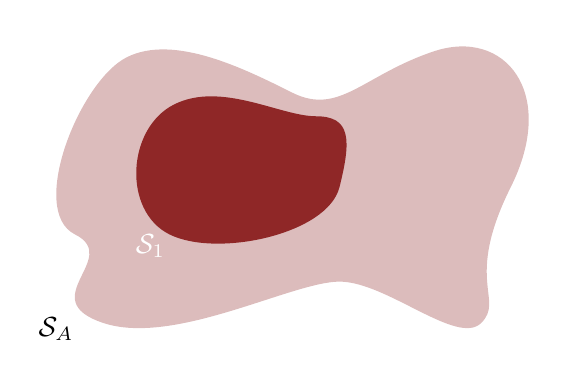
\begin{tikzpicture}[scale=0.3, thick] 
  \pgfmathsetmacro{\dx}{-27}
  %\draw [rounded corners=2pt, color=black] (-10 + \dx, -6) rectangle (10 + \dx, 6);
 
  %\fill [color=light] (-9.2 + \dx, -2) 
  %                   .. controls (-11.2 + \dx, -1) and (-9 + \dx, 4.5) .. (-7 + \dx, 5.5) 
  %                   .. controls (-5 + \dx, 6.5) and (-2 + \dx, 5) .. (0 + \dx, 4)
  %                   .. controls (2 + \dx, 3) and (3 + \dx, 4.75) .. (6 + \dx, 5.75) 
  %                   .. controls (9 + \dx, 6.75) and (11.25 + \dx, 4) .. (9.25 + \dx, 0)
  %                   .. controls (7.25 + \dx, -4) and (9 + \dx, -4.75) .. (8 + \dx, -5.75) 
  %                   .. controls (7 + \dx, -6.75) and (4 + \dx, -4) .. (2 + \dx, -4)
  %                   .. controls (0 + \dx, -4) and (-5 + \dx, -6.75) .. (-8 + \dx, -5.75) 
  %                   .. controls (-11 + \dx, -4.75) and (-7.2 + \dx, -3) .. (-9.2 + \dx, -2);
           
  %\draw [->, >=stealth, line width=10, color=black] (-16, 0) -- +(5, 0);
        
  %\node [] at (-10 + \dx, -6) { $\mathcal{S}_{A}$ };
                     
  \pgfmathsetmacro{\dx}{0}
  %\draw [rounded corners=2pt, color=black] (-10 + \dx, -6) rectangle (10 + \dx, 6);
 
  \fill [color=light] (-9.2 + \dx, -2) 
                     .. controls (-11.2 + \dx, -1) and (-9 + \dx, 4.5) .. (-7 + \dx, 5.5) 
                     .. controls (-5 + \dx, 6.5) and (-2 + \dx, 5) .. (0 + \dx, 4)
                     .. controls (2 + \dx, 3) and (3 + \dx, 4.75) .. (6 + \dx, 5.75) 
                     .. controls (9 + \dx, 6.75) and (11.25 + \dx, 4) .. (9.25 + \dx, 0)
                     .. controls (7.25 + \dx, -4) and (9 + \dx, -4.75) .. (8 + \dx, -5.75) 
                     .. controls (7 + \dx, -6.75) and (4 + \dx, -4) .. (2 + \dx, -4)
                     .. controls (0 + \dx, -4) and (-5 + \dx, -6.75) .. (-8 + \dx, -5.75) 
                     .. controls (-11 + \dx, -4.75) and (-7.2 + \dx, -3) .. (-9.2 + \dx, -2);
                     
  \fill [color=dark] (-5.2 + \dx, -2) 
                     .. controls (-7.2 + \dx, -1) and (-7 + \dx, 2.5) .. (-5 + \dx, 3.5) 
                     .. controls (-3 + \dx, 4.5) and (-0.5 + \dx, 3) .. (1 + \dx, 3)
                     .. controls (2.5 + \dx, 3) and (2.5 + \dx, 2) .. (2 + \dx, 0)
                     .. controls (1.5 + \dx, -2) and (-3.2 + \dx, -3) .. (-5.2 + \dx, -2); 
                     
  \node [] at (-10 + \dx, -6) { $\mathcal{S}_{A}$ };
  \node [color=white] at (-6 + \dx, -2.5) { $\mathcal{S}_{1}$ };
         
\end{tikzpicture}

\end{document}   